\section{Outline}
Following is the outline of the paper.

 \subsection{Introduction}

\subsection{Audio performance measurement of smartphone}

Speaker and Mic lobes. Their frequency response. Audio lobe reflection measurement. An-echoic chamber. How much distance we can measure ? Reflected signal strength vs different material vs sound level vs (if possible) different phone. 

Different false starts. Pulse/Echo based method. Moving around a single space won't work.

\subsection{Problem statement}
Path profiling combined with distance measurement. Different sub-challenges and how to address them:

\begin{itemize}
\item Accurate dead-reckoning.
\item Audio lobe intensity.
\item FMCW accuracy measurement.
\item Combating different multi-path.
\item Corner detection.
\item Small thing or clutter detection.
\item Geometric ambiguity removal to create contour.
\end{itemize}

We moved forward with the following building blocks:
\begin{itemize}
\item Single wall contour.
\item Multi-wall contour.
\item Multi-wall contour with clutter presence or with different path profile.
\end{itemize}

\subsection{Design and Observations}

\subsubsection{Different False Attempts or Starts}
\begin{itemize}
\item Pulse based echo selection and finding or Echo-sorting (Too much direct path impact).
\item Angle-of-arrival calculation (Too less number of mics and sine based or CIR based phase measurement won't work due to high level of multi-path).
\item MUSIC based peak selection (Prior knowledge of number of peaks).
\end{itemize}

\subsubsection{FMCW based observations}
\begin{itemize}
\item Junction causes mutliple peaks.
\item Maximum peak in FMCW corresponds to the main wall distance.
\item Always get perpendicular distance from wall.
\item Peak amplitude increases with the size of the reflector and it saturates after certain size.
\item Corner peaks are significantly different (at least for corner less than or equal to 90 degree). There are multiple peaks and peak spread is more.
\item Audio lobe direction and mic position matters.
\end{itemize}

\subsection{Methodology or Algorithm}
Description of the algorithm and geometric arguments with some explanatory figures. Fig.~\ref{fig:roomshape_algo} illustrates the algorithm used in room shape detection.

\begin{figure}[h!t]
\center{
\fbox{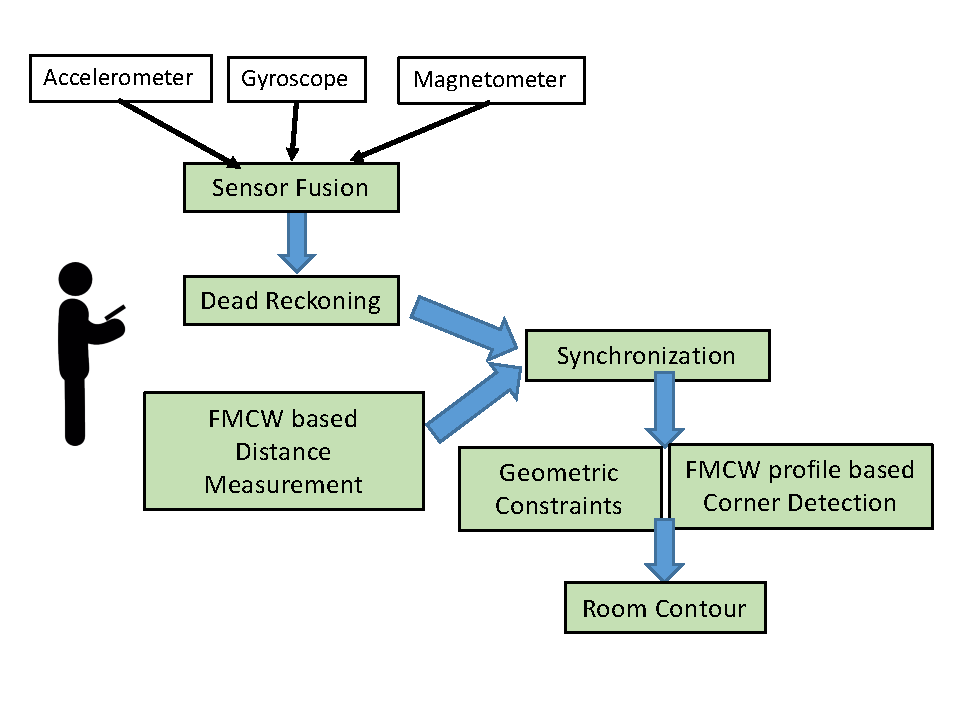
\includegraphics[width=\columnwidth]{figs/roomshape_algo.pdf}}
\caption{Algorithm sketch of \textit{Batphone}}
\label{fig:roomshape_algo}
}
\end{figure}

\subsubsection{Dead Reckoning}
\begin{itemize}
\item Step size estimation
\item Step detection and count
\item Heading direction
\item Phone orientation
\end{itemize}

\subsubsection{FMCW based distance}
\begin{itemize}
\item FMCW parameter choices ( Chirp duration, Mic choice, Frequency response of speaker and mic based selection, Gap between chirps, Bandwidth selection, Sampling rate selection (Higher means lower quantization error or can also be done with zero padding). )
\item Synchronization with dead reckoning.
\item FMCW profile based corner detection and clutter filtering.
\end{itemize}

\subsubsection{Room shape profiling}
\begin{itemize}
\item Geometric constraints on the room wall and movement.
\item Corner detection help in profiling.
\end{itemize}


\subsection{Evaluation}
\subsubsection{Micro-benchmark for FMCW}

1) Micro-benchmark on FMCW based distance measurement :
 
    - Different distance measurement accuracy

    - Wall orientation w.r.t path of the phone accuracy

 - Also vary the distance from the wall as this impacts the accuracy
 
    - Resolution of distance measurement accuracy

how do you plan to evaluate this? 

    - Reflector size vs Distance measurement
  
    - Phone Orientation

   - Impact of phone height (peaks from ceiling + floor) and phone holding pattern

   - Path profiling error (accelerometer + gyro)
   
[Put some experiment images, anechoic chamber images etc.]

\subsubsection{Single wall Contour}

  - Different shape (Round vs Straight) or Triangle vs Round

   - Also need to try more shapes and sizes

\subsubsection{Multi wall Contour}

  Corner detection accuracy (False positive rate)
   
  - Different angles
 
  - Different sized walls in intersection
  
  - Direction association accuracy (If you are moving along a straight line and you have one wall in right or left side. How do you know which side is your wall ?)
  
\subsubsection{Multi wall Contour with clutter}

Sensitivity to surrounding small objects by trying to add different sizes small objects at different locations to see if you can effectively filter them out 

[We may have to leave profiling the small objects to the future work. For this work, we just aim to filter them out.]

\subsubsection{Motion Planning}
8) motion planning 

For a given environment, how can different motion planning (random, or moving constant steps along each object, or dynamically adjusting the steps based on the imaging results) perform in terms of imaging qualities and distance travelled.


\subsection{Points of discussion}
Some small discussions.

\subsection{Related work}
Some related work.

\subsection{Conclusion and Future work}
Here we conclude.



